% !TEX program = xelatex
% Example: PGFPlots function plot
\documentclass[11pt, a4paper]{article}
\usepackage{pgfplots}
\pgfplotsset{compat=1.18}

\begin{document}

\section*{رسمُ الدوالِّ بـ PGFPlots}

% رسمُ دالتين على نفسِ المحاور
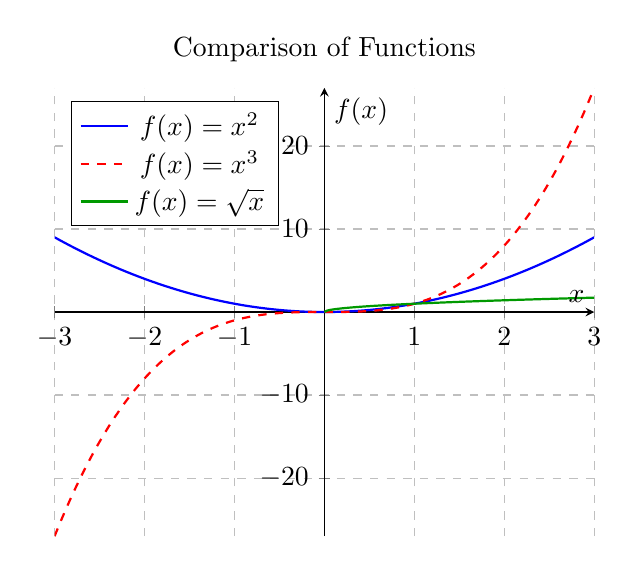
\begin{tikzpicture}
\begin{axis}[
  xlabel={$x$},
  ylabel={$f(x)$},
  title={Comparison of Functions},
  legend pos=north west,
  grid=major,
  grid style=dashed,
  axis lines=middle
]
  \addplot[blue, thick, domain=-3:3, samples=100] {x^2};
  \addlegendentry{$f(x) = x^2$}

  \addplot[red, thick, dashed, domain=-3:3, samples=100] {x^3};
  \addlegendentry{$f(x) = x^3$}

  \addplot[green!60!black, thick, domain=0:3, samples=100] {sqrt(x)};
  \addlegendentry{$f(x) = \sqrt{x}$}
\end{axis}
\end{tikzpicture}

\end{document}
